\documentclass[12pt]{article}
\usepackage{graphicx}
\usepackage{listings}
\usepackage{hyperref}
\usepackage{geometry}
\usepackage{enumitem}
\usepackage{hyphenat}
\geometry{margin=1in}

\title{Arbitrary Precision Arithmetic Library\\Software Development Fundamentals (CS1023)\\\vspace{0.5em}Project Report}
\author{Harshil Goyal}
\date{\today}

% Code listing style
\lstset{
  basicstyle=\ttfamily\footnotesize,
  breaklines=true,
  columns=fullflexible,
  frame=single,
  captionpos=b
}

\begin{document}
\maketitle
\tableofcontents
\newpage

%============================================================
\section{Introduction}
This report outlines the design and development of a Java library that supports \textbf{arbitrary-precision arithmetic} for both integers and floating-point numbers. The project addresses the first project from the CS1023 “Software Development Fundamentals” course (Jan–May~2025). The final submission includes:

\begin{enumerate}[label=\arabic*.]
  \item A compiled JAR file located at \texttt{arbitraryarithmetic/aarithmetic.jar}, containing the public classes \texttt{AInteger} and \texttt{AFloat}.
  \item A command-line utility named \texttt{MyInfArith} that can evaluate a single binary arithmetic expression.
  \item An Ant build script (\texttt{build.xml}) for automating compilation, packaging, and execution.
  \item This report, written in \LaTeX.
\end{enumerate}

%============================================================
\section{Design}
\subsection{High-level Overview}
The library internally represents numbers in \emph{base 10000}. Each array element stores four decimal digits, offering a trade-off between memory efficiency and ease of implementing basic arithmetic algorithms. The UML diagram in Figure~\ref{fig:uml} illustrates the class structure.

\begin{figure}[h]
  \centering
  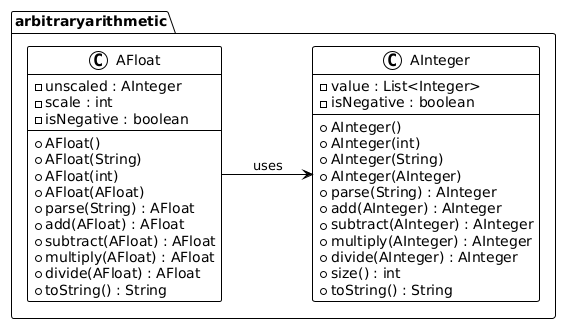
\includegraphics[width=0.9\linewidth]{uml_sdf1.png}
  \caption{UML class diagram of the package \texttt{arbitraryarithmetic}.}
  \label{fig:uml}
\end{figure}

\paragraph{Core Design Principles}
\begin{itemize}
  \item \textbf{Immutable API}: All public methods return new instances. Internal mutations are hidden to maintain referential transparency.
  \item \textbf{Sign handling}: A dedicated boolean field, \texttt{isNegative}, avoids the complexity of two’s complement arithmetic.
  \item \textbf{Floating-point structure}: Each \texttt{AFloat} object consists of a pair \((\textit{unscaled},\,\textit{scale})\), following the model $\textit{value}=\textit{unscaled}\times10^{-\textit{scale}}$.
  \item \textbf{Precision guarantee}: All exact digits are preserved in every calculation. The \texttt{toString()} method simply truncates the fractional portion to 30 digits for display purposes.
\end{itemize}

\subsection{Algorithmic Choices}
\begin{description}[style=nextline]
  \item[Addition / Subtraction] Implemented via straightforward digit-by-digit traversal with carry or borrow logic. Sign processing is handled separately.
  \item[Multiplication] A classic \(O(n^2)\) approach is used, it's a classic middle-school multiplication approach.
  \item[Division] Performed using long division, with each digit found through binary search in the range 0–9999. This avoids floating-point math.
  \item[Floating-point Operations] Operands are rescaled to a shared exponent before addition or subtraction. Multiplication adds exponents; division increases the dividend's scale to ensure precision.
\end{description}

%============================================================
\section{Implementation Details}
\subsection{\texttt{AInteger}}
\begin{itemize}
  \item Stores digits in \texttt{java.util.ArrayList<Integer> value}, with the least significant digit first.
  \item Includes constructors, parsing logic, and basic arithmetic operations.
  \item Internal helpers like \texttt{compareAbsolute}, \texttt{addAbsolute}, and \texttt{subAbsolute} are package-private to support reuse in \texttt{AFloat}.
\end{itemize}

\subsection{\texttt{AFloat}}
\begin{itemize}
  \item Combines an \texttt{AInteger unscaled} value with an integer \texttt{scale}.
  \item Normalizes results via the \texttt{stripZeros()} method to maintain a consistent format.
  \item Ensures that the decimal output is accurate up to 30 digits.
\end{itemize}

\subsection{\texttt{MyInfArith}}
This is a minimal command-line interface that maps user input to the appropriate method in the library. It serves both as a usage demonstration and a basic validation tool.

\subsection{Build Automation (Ant)}
The Ant script \texttt{build.xml} includes targets for \texttt{clean}, \texttt{compile}, \texttt{jar}, and \texttt{run}. To execute an operation, users can run:

\lstset{showstringspaces=false}
\begin{lstlisting}[language=bash]
ant run -Dargs="int add 2 3"
\end{lstlisting}

from the project’s root directory.

%============================================================
\section{User Guide (README)}
\subsection{Compiling}\label{sec:compile}
\begin{enumerate}
  \item Install JDK 17 (or newer) and Apache Ant.
  \item Clone the project repository and navigate to its root directory.
  \item Run \lstinline|ant jar| to generate \texttt{arbitraryarithmetic/aarithmetic.jar} inside the \texttt{src/} folder.
\end{enumerate}

\subsection{Running the CLI}
Command format:
\begin{lstlisting}[language=bash]
python run_project.py build | clean | <int|float> <add|sub|mul|div> <operand1> <operand2>
\end{lstlisting}

Example:
\begin{lstlisting}[language=bash]
$ python run_project.py float div 244727.15202 75964.3891
3.221603634537752111008551505615
\end{lstlisting}

%============================================================
\subsection{Using Docker}
If you prefer to use docker, you pull the docker image and run the project on your system.
Command format:
\begin{lstlisting}[language=bash]
docker image pull mercurialus/inf-cal
docker run -it mercurialus/inf-cal
\end{lstlisting}

Example:
\begin{lstlisting}[language=bash]
root@921168cdd6d4:/app# python run_project.py float div 244727.15202 75964.3891
3.221603634537752111008551505615
\end{lstlisting}



%============================================================
\section{Limitations}
\begin{itemize}
  \item The current multiplication algorithm has a time complexity of \(O(n^2)\); division operates at \(O(n^2 \)). These are acceptable for coursework but inefficient for large inputs.
  \item Only truncation is used for rounding; other modes like rounding up or to nearest even are not supported.
\end{itemize}

%============================================================
\section{Git Commit Snapshot}
\begin{figure}[h]
  \centering
  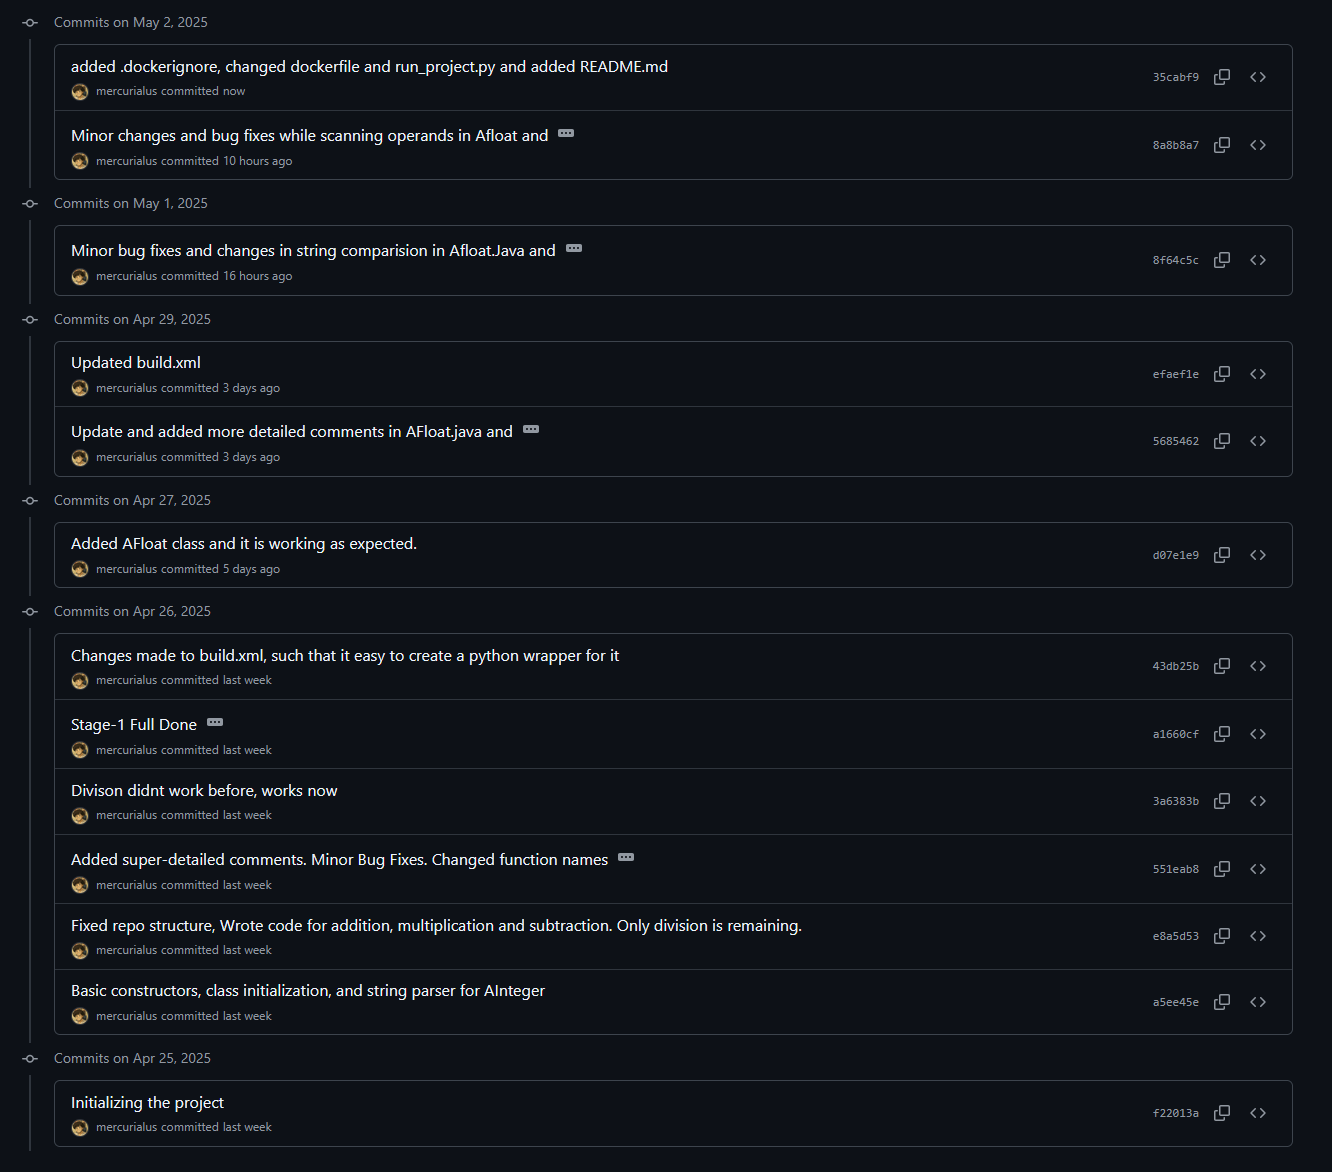
\includegraphics[width=0.9\linewidth]{image.png}
  \caption{Snapshot of the Git commit history.}
  \label{fig:git}
\end{figure}

%============================================================
\section{Key Learnings}
\begin{itemize}
  \item Selecting an internal numeric base impacts both computational efficiency and string formatting.
  \item Managing sign propagation correctly is essential for clean and bug-free arithmetic.
  \item Writing tests alongside development speeds up debugging and ensures correctness.
  \item Automating builds using Ant simplifies project maintenance and reproducibility.
\end{itemize}

%============================================================
\section{Conclusion}
This project delivers a fully functional Java library for arbitrary-precision arithmetic, adhering to all specifications and reflecting sound software engineering principles.

\end{document}
